\section{Параллельные алгоритмы~-- i (Осипов Д.)}

Неформально говоря, {\bfseries параллельный алгоритм}~-- это алгоритм, который может использовать несколько процессоров одновременно.
\subsection{Булевы схемы}
\begin{definition*}
	{\bfseries Булева схема}~-- ориентированный граф без циклов, где:
\begin{itemize}
    \item вершины без входящих ребер соответствуют входным данным,
    \item вершины с входящими ребрами (<<гейты>>) помечены исполняемыми в них булевыми операциями,
    \item некоторые вершины помечены как <<выходы>>, то есть соответствуют выходным данным.
\end{itemize}
Булева схема вычисляет функцию, определяемую естественным образом (операции последовательно
применяются к тем данным, которые приходят по входящим рёбрам).
\end{definition*}
\begin{example*}
$ $
    \begin{center}
    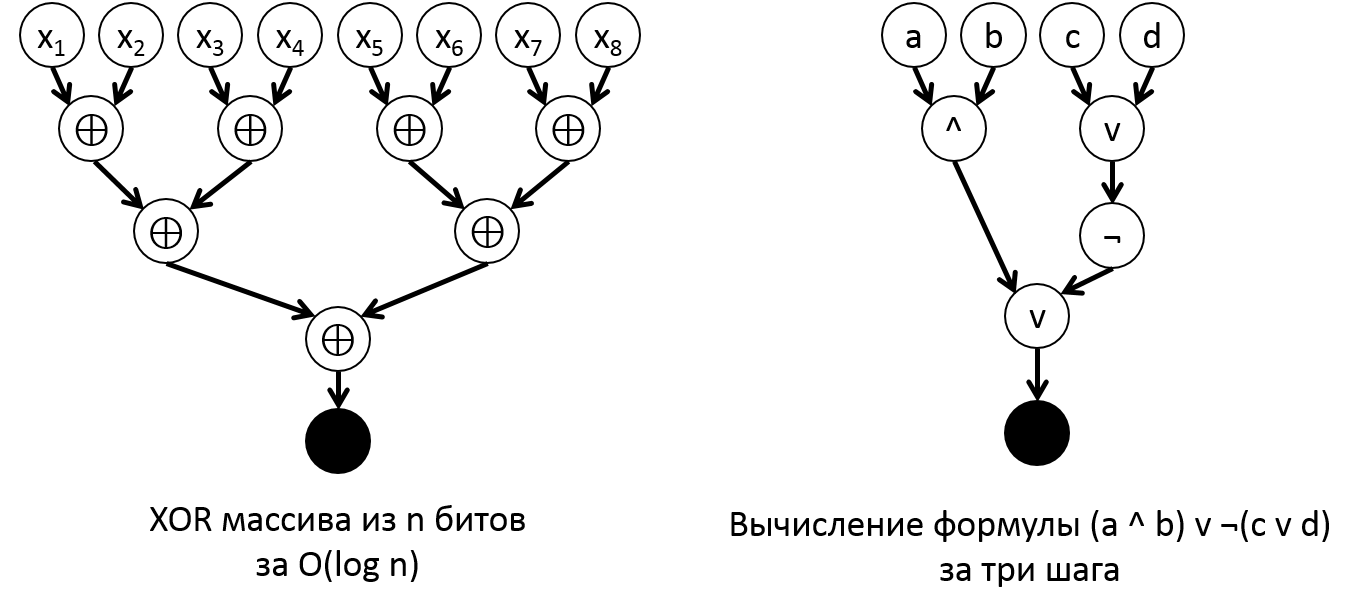
\includegraphics[scale=0.5]{figures/boolex.png}
    \end{center}
\end{example*}

Если значение в вершине не зависит от значения, вычисляемого в другой вершине, то
операции в этих вершинах могут исполняться в любом порядке, в том числе одновременно.
Поэтому булевы схемы являются удобной моделью параллельных вычислений:
каждой вершине соответствует свой процессор, который выполняет только операцию, соответствующей данной вершине.

\begin{definition*}
Параллельное время работы алгоритма, представленного булевой схемой,
равно
\textit{<<глубине>>} схемы, т.е. длине самого длинного пути от вершины до выхода.
\end{definition*}

Количество необходимых процессоров на самом деле можно уменьшить.
Заметим, что если каждому гейту присвоить число~-- <<номер этажа>> так, что каждый переход осуществляется с <<верхнего>> этажа на <<нижний>>, то максимальное число процессоров на одном этаже~-- достаточное количество процессоров для исполнения всего алгоритма. Так, в левом примере достаточно взять четыре процессора, а в правом~-- два.
Формально можно было бы определить параллельную версию RAM-машины (PRAM),
но в данном курсе мы этого делать не будем,
а ограничимся естественным пониманием многопроцессорной машины
(в частности, наши алгоритмы будут построены таким образом, что
конфликтов из-за одновременного чтения и/или записи
в одно место общей памяти не будет возникать).
Основной нашей формальной моделью вычислений останутся булевы схемы.

Вычисление XOR массива за $O(\log n)$ параллельных шагов в примере слева~-- уже хороший пример параллельного алгоритма. Хотя он интуитивно понятен, опишем его формально.

\begin{problem*}
	Пусть дано $n$ битов. Вычислить их XOR.
\end{problem*}

\begin{algodescription}{Решение за $O(\log n)$} Считаем, что $n$~-- степень двойки (если нет, дополним нулями).  Разобъем все числа на $n/2$ пар и поручим каждому процессору одну пару, чтобы он вычислил ее сумму. Получившиеся $n/2$ чисел разобъем на $n/4$ пар и так же вычислим суммы этих пар. Повторяем до тех пор, пока не останется одно число. Ясно, что всего будет выполнено $\log_2 n = O(\log n)$ параллельных шагов.
\end{algodescription}

\begin{nb*} $\heart$ Сложить\footnote{Имея в распоряжении только <<+>>-гейты, принимающие ровно два числа} $n$ чисел быстрее, чем за $\log n$ шагов, нельзя. В самом деле, если можно, то булева схема такого алгоритма как граф-дерево имеет высоту $h \leq \log_2 n - 1$. Но каждый гейт принимает на вход не больше двух чисел, т.е. входная степень каждой вершины не больше 2. Значит верхних входных гейтов не может быть более $2^h \leq n/2$  чисел, а надо $n$.
\end{nb*}

При проектировании параллельных алгоритмов в качестве меры их эффективности возникает аж три параметра: \textit{количество параллельных шагов (время работы)}, \textit{количество используемых процессоров} и \textit{общая работа} (определение дано далее). К счастью, об одном из них~-- количестве процессоров~-- можно не задумываться, о чем говорит нам следующее утверждение.

\subsection{Принцип Брента}
\begin{theorem*}[принцип Брента]
	Рассмотрим параллельный алгоритм, выполняющий t параллельных шагов, где на $i-$м шаге задействовано $w_i$ процессоров (т.е. выполняется $w_i$ операций). Обозначим $W=\sum\limits_{i=1}^t w_i$ и назовем эту величину \underline{общей работой алгоритма} (это количество гейтов в булевой схеме). Тогда алгоритм можно перепрограммировать так, чтобы на $P$ процессорах он работал не более, чем за $\frac{W}{P} + t$ параллельных шагов. \emph{NB: здесь имеется в виду количество шагов, выполняемых какой-то многопроцессорной машиной, а не параллельное время, которое мы определили формально как глубину булевой схемы.}
\end{theorem*}

\begin{proof}
	Перераспределим все $W$ операций на $P$ процессоров наиболее равномерно, разбив $i$-й шаг изначального алгоритма на $\left\lceil\frac{w_i}{P}\right\rceil$ новых шагов. Оценим общее число шагов нового алгоритма:
$$t' = \sum_{i=1}^t \left\lceil\frac{w_i}{P}\right\rceil \leq \sum_{i=1}^t \left(\frac{w_i}{P} + 1\right) = \sum_{i=1}^t \frac{w_i}{P} + t = \frac{W}{P} + t$$Таким образом, получили алгоритм с искомым временем работы.
\end{proof}

\begin{nb*} Принцип Брента позволяет при проектировании параллельных алгоритмов \textbf{не думать}, на скольких процессорах будет работать алгоритм. Именно: пусть был создан алгоритм, работающий на неизвестном (лень считать) числе процессоров $P_0(n)$ и совершающий общую работу $W(n)$ за $t(n)$ параллельных шагов. Тогда его можно перепроектировать на любое число процессоров $P(n)$ такое, что $$\frac{W(n)}{P(n)} = O(t(n)),$$ и асимптотически не потерять во времени, так как тогда новое время работы все еще $t'(n) \leq \frac{W(n)}{P(n)} + t(n) = O(t(n))$. Даже если у нас есть меньшее количество процессоров, мы можем запустить на них этот алгоритм с соответствующей потерей по времени (а вот большее количество процессоров никакого гарантированного выигрыша не даёт). Поэтому в дальнейшем при изучении параллельных алгоритмов мы оптимизируем время работы, а не число процессоров, и считаем, что у нас \textbf{сколь угодно много процессоров}, количество нужных процессоров можно вычислить по принципу Брента.
\end{nb*}

\subsection{Параллельное умножение булевых матриц}
\begin{nb*}
    Мы перемножаем здесь именно булевы матрицы только для того, чтобы было просто рисовать булевы схемы.
    Аналогичным образом можно перемножить любые матрицы, но элементарные операции (например, сложение чисел)
    надо будет заменить на подсхемки, которые их вычисляют.
\end{nb*}

\begin{problem*}
	Даны две битовые матрицы $A$ и $B$ размера $n\times n$. Вычислить их произведение, то есть числа $C_{ij} = \bigvee_{k=1}^n A_{ik}\land B_{kj}$  для всех $i, j=1\ldots n$ (всего $n^2$  чисел).
\end{problem*}

\begin{algodescription}{Непараллельное решение}
    Вычислить все $n^2$ чисел $C_{ij}$, каждое считается за $O(n)$, значит общая сложность $O(n^3)$.
    В первой части курса был более быстрый алгоритм, но все равно быстрее $O(n^{2.\ldots})$
    никто не умеет решать эту задачу, а уж тем более - за $O(\log n)$.
\end{algodescription}

Несмотря на то, что в прошлом разделе мы условились не думать о количестве процессоров, конкретно здесь на всякий случай приведем два решения. Второе решение~-- просто пример того, как работает принцип Брента.

\begin{algodescription}{Решение за $O(\log n)$ времени на $n^3$ процессорах}
    Занумеруем все $n^3$ процессоров тройками чисел $(i, k, j)$, где $i,k,j=1\ldots n$. Сначала на каждом процессоре $(i, k, j)$ посчитаем $A_{ik}\land B_{kj}$. Теперь хотим получить число $C_{ij} = \bigvee_{k=1}^n (i, k, j)$, Сделаем это за $\log n$ шагов (бинарным деревом). Задача решена за $1+\log n = O(\log n) $ шагов на $n^3$ процессорах.
\end{algodescription}

Общая работа этого решения $W(n) = O(n^3)$. Действительно, ведь данное решение просто считает $n^2$ выражений $C_{ij} = \bigvee_{k=1}^n A_{ik}\land B_{kj}$, расставив скобки внутри большой дизъюнкции, таким образом, $n^2$ раз совершено $n$ действий дизъюнкций. Тогда из принципа Брента следует, что для исполнения этого алгоритма за $O(\log n)$ на самом деле достаточно $P(n) = \frac{W(n)}{t(n)} = O\left(\frac{n^3}{\log n}\right)$ процессоров.

Можно даже явно перепроектировать алгоритм, чтобы он работал на $O\left(\frac{n^3}{\log n}\right)$ процессорах.

\begin{algodescription}{Решение за $O(\log n)$ времени на $O\left(\frac{n^3}{\log n}\right)$ процессорах} Модифицируем алгоритм выше. На первом шаге вычислить все числа $A_{ik}\land B_{kj}$ получится не за 1, а за $O(\log n)$ шагов: за каждый шаг просто посчитаются очередные $\frac{n^3}{\log n}$ чисел $A_{ik}\land B_{kj}$. Получать из них $C_{ij}$ за $O(\log n)$ мы уже умеем. Итоговая сложность $O(\log n) + O(\log n) = O(\log n)$.
\end{algodescription}

\subsection{Параллельная достижимость в графе}
\begin{problem*}
	Дан граф, заданный матрицей смежности $\{a_{ij}\}$. Построить его матрицу достижимости.
\end{problem*}

\begin{algodescription}{Решение за $O(\log^2 n)$ времени} Будем булево умножать матрицы: вместо $\cdot$ возьмем $\land$, вместо $+$ возьмем $\lor$. Из формулы перемножения матриц несложно видеть, что $A^k$~-- матрица $k-$шаговой достижимости. Тогда матрица достижимости~-- любая матрица $A^k$, где $k\geq n$. Умеем возводить матрицу в квадрат за $O(\log n)$. Для получения матрицы достижимости $A^n$. возведем матрицу $A$ в квадрат $\log n$ раз. Итоговая сложность $O(\log n) \cdot O(\log n) = O(\log^2 n)$. Общая работа $W(n) = O(n^3\log n)$, так как $\log n$ раз перемножили матрицы за $O(n^3)$ работы. Число процессоров: $P(n) = O\left(\frac{n^3\log n}{\log^2 n}\right) = O\left(\frac{n^3}{\log n}\right)$.
\end{algodescription}
